\chapter{Numerical Simulations} \label{Chp:sim}
\chaptermark{Numerical Simulations}

Numerical simulation has been an important tool in \acs{MRI} because unexpected errors due to system imperfections (e.g.~eddy currents, noise, and field inhomogeneities) and uncooperative patients (e.g.~through-plane motions) can be excluded. Moreover, it creates an ideal imaging environment that fosters understanding the characteristics of different k-space sampling trajectories and evaluating reconstruction methods. Therefore, a simulation framework based on analytical Fourier transformation is built for the studies of various radial sampling schemes, e.g.~asymmetric-echo and multi-echo radial \acs{FLASH}.

\section{Fundamentals}
In principle, the MR signal in k-space is the continuous Fourier transform of the scanned object $\rho(\vec{r})$, which can be written as 
\begin{equation} \label{Equ:cont_FT_rho}
y(t) = \int_{\vec{r}} \rho(\vec{r}) \cdot e^{-i 2\pi \cdot \vec{k}(t) \cdot \vec{r}} \text{d} \vec{r}
\end{equation}

One typical MR simulation was based on rasterized phantoms, and the MR signal was obtained via discrete Fourier transform (\acs{DFT}). This approach, however, is time consuming as every k-space signal requires an execution of DFT over all image pixels. Nevertheless, it leads to the inverse-crime problem, as the same discrete model of the imaging system is used for both simulation and image reconstruction. Moreover, the MR signal from a rasterized phantom can not represent the aliasing artifact from truncated k-space. Therefore, it is more reliable and preferable to use analytical phantoms with three important features.

First of all, the analytical Fourier transform of phantoms constructed by superimposed ellipses and rectangles (e.g.~Shepp-Logan phantom \cite{1974_SL,2008_SL_Gach}) can be derived as
\begin{align} 
  A_{\text{circ}}(k_x,k_y) &= a \cdot b \cdot \frac{J_1(\sqrt{(a \cdot k_x)^2 + (b \cdot k_y)^2})}{\sqrt{(a \cdot k_x)^2 + (b \cdot k_y)^2}} \label{Equ:aFT_circ} \\
\intertext{and}
  A_{\text{rect}}(k_x,k_y) &= 2\pi \cdot a \cdot b \cdot \sinc(a \cdot k_x) \cdot \sinc(b \cdot k_y) \label{Equ:aFT_rect}
\end{align}
respectively \cite{2008_Block_Thesis}. Here, $J_1(x)$ is the first-order Bessel function of its first kind, $a$ and $b$ represent either the short and long axes of an ellipse, or the length and width of a rectangle. On the other hand, due to the linearity of Fourier transform, superimpositions in image domain are equivalent to those in k-space. Therefore, the analytical Fourier transform of any phantom with superimposed ellipses and/or rectangles can be calculated given the sampling k-space trajectory, which is given as
\begin{equation} \label{Equ:sum_aFT_rho}
  y(\vec{k}) = \sum_{m} I_m \cdot A_m(\vec{k})
\end{equation}
with $m$ being the index for ellipses and rectangles in the phantom, and $I_m$ and $A_m$ the corresponding proton density and analytical Fourier transform, respectively.

Secondly, the inclusion of multiple spatially-varying receiver coils $c_j(\vec{x})$ to mimic parallel imaging, which extends the MR signal in \cref{Equ:cont_FT_rho} to 
\begin{equation} \label{Equ:cont_FT_rho_coil}
  y_j(t) = \int_{\vec{r}} c_j(\vec{r}) \cdot \rho(\vec{r}) \cdot e^{-i 2\pi \cdot \vec{k}(t) \cdot \vec{r}} \text{d} \vec{r} \quad .
\end{equation}
With sinusoidal or polynomial fitting of the complex coil sensitivity map simulated from Biot-Savart law, the fitting coefficients can be integrated into the analytical Fourier transform of phantoms. Mathematical description of the integration procedure is given in \cref{Chp:AnalCoil}.

Thirdly, the inclusion of relaxation effects (e.g.~\acs{T2s} signal decay and off-resonance phase modulation in multi-echo FLASH) into the MR signal model, which is further extended from \cref{Equ:cont_FT_rho_coil} to
\begin{equation} \label{Equ:cont_FT_rho_coil_ME}
  y_{j,l}(t) = \int_{\vec{r}} c_j(\vec{r}) \cdot \rho(\vec{r}) \cdot e^{-[R_2^*(\vec{r}) + i 2\pi \cdot \Delta f (\vec{r})] \cdot \text{TE}_l} \cdot e^{-i 2\pi \cdot \vec{k}(t) \cdot \vec{r}} \text{d} \vec{r}
\end{equation}
where $R_2^*$ is the reciprocal of the $T_2^*$ relaxation time, $\Delta f$ is the off-resonance frequency map, and $\text{TE}_l$ is the echo time of the $l$\textsuperscript{th} echo. The relaxation effects can be included by assuming $T_2^*$ and $\Delta f$ values in every shape (ellipse or rectangle) to be constant, so that the MR signal in accordance to \cref{Equ:sum_aFT_rho} is (ignoring the coil sensitivities for simplicity)
\begin{equation} \label{Equ:sum_aFT_rho_relax}
  y_l(\vec{k}) = \sum_{m} I_m \cdot e^{-z_m \cdot \text{TE}_l} \cdot A_m(\vec{k})
\end{equation}
with $z_m = R_2^* + i 2\pi \cdot \Delta f$. One drawback of this method is that off-resonances are constant within a shape and hence discrete in a phantom, which does not reflect the fact that off-resonance frequency maps are usually smooth and slowly-varying in space, similar to coil sensitivity maps. This drawback, however, can be overcome using approximation methods as for coils.

Using the analytical phantom with the above features, a numerical simulation framework was developed in MATLAB (Mathworks, Natick, MA, IUSA) for studying the characteristics of different radial sampling schemes.

\section{In-Plane Motion Simulations}
To study motion artifacts in real-time MRI, to mimic the experimental motion phantom \cite{2013_MotionPha}, and to test motion-correction algorithms (e.g.~application of k-space energy spectrum analysis to motion correction in \acs{PROPELLER} MRI \cite{2006_KESA,2012_KESA_Tan}), this simulation framework is capable of adding in-plane motions (e.g. translation and rotation) to every acquired k-space spoke. 

The principle of motion simulation is that the geometries of all shapes contained in a phantom (i.e., the center, the major and minor semi-axes of a ellipse) are consistent during the acquisition of a spoke, and thus the k-space signal of this spoke can be calculated by analytical Fourier transform given the known geometries. The geometries can then be changed for the acquisition of the next spoke. Taking in-plane rotation as an example, the centers of the two tubes are updated every spoke by rotating the tubes around the center of the imaging slice according to the user-defined rotation angle per spoke. Note that the rotation angle can be converted to the rotation speed (\si{\cm\per\second}) as used in the experimental motion phantom,
\begin{equation} \label{Equ:rot_speed}
v = \phi \cdot d / T
\end{equation}
where $\phi$ is the rotation angle per frame, $d$ the distance from the center of the tube to that of the rotation, and $T$ the acquisition time for one image. Therefore, the rotation angle of \ang{5.7} per frame in \cref{Fig:sim-motion-halfPos} corresponds to half-position shift and \SI{15}{\cm\per\second} for the outer tube. As the distance to the image center from the outer tube is twice as long as the inner one, the outer tube rotates twice as fast and hence it suffers from more severe blurring. 

Furthermore, to prove the temporal acuity of NLINV without the temporal median filter, \cref{Fig:sim-motion-comp} compares it with the conventional Gridding \& FFT reconstruction \cite{1991_conv_gridding,2005_gridding}. Firstly, as shown in the static phantom images, NLINV can greatly suppress streaking artifacts due to undersampling as it iteratively estimates the optimal image that matches best with the acquired k-space data, while Tikhonov regularization on the image penalizes unwanted signals from high-spatial-frequency area, i.e., noise and streaks. Secondly, the rotation angle per frame \ang{5.7}, \ang{11.4}, and \ang{17.1} corresponds to the rotation speed of \SI{15}{\cm\per\second}, \SI{30}{\cm\per\second} and \SI{45}{\cm\per\second} for the outer tube, respectively. The resulting images from Gridding \& FFT reconstruction are degraded by heavier spatial discontinuity along with higher rotation speed, while images from NLINV show blurring artifacts because NLINV for serial images relies on the temporal regularization, which could be explored to find an optimum for rapid-motion imaging, i.e. \SI{45}{\cm\per\second}. The optimization of the regularization parameters, however, is beyond the scope of this chapter.

In short, these simulation results match the findings from real-time MRI on the experimental motion phantom \cite{2014_Temp_Fidelity}.
\begin{figure}[tb]
  \centering
  \includegraphics[width=\textwidth]{fig/sim-motion-halfPos.png}
  \caption{Eight consecutive images (from the \nth{43} to \nth{50} frame) with an in-plane rotation of $5.7^o$ per frame in the clockwise direction, base resolution 200, FOV \SI{20}{\square\cm}, \num{17} spokes per frame (\SI{33}{\ms} temporal resolution), \num{5} interleaves, \ang{360} total view angle, and \num{10} analytical coils. The images were reconstructed by NLINV without the temporal median filter.} \label{Fig:sim-motion-halfPos}
\end{figure}

\begin{figure}[tb]
  \centering
  \includegraphics[width=\textwidth]{fig/sim-motion-comp.png}
  \caption{Comparisons of (top) Gridding \& FFT and (bottom) NLINV reconstructions under different rotation speeds: (1\textsuperscript{st} column) stationary, (2\textsuperscript{nd} column) \ang{5.7} per frame, (3\textsuperscript{rd} column) \ang{11.4} per frame, and (4\textsuperscript{th} column) \ang{17.1} per frame. The other acquisition parameters are identical to those in \cref{Fig:sim-motion-halfPos}.} \label{Fig:sim-motion-comp}
\end{figure}
